\documentclass[10pt,pdf]{beamer}
\usepackage[T2A]{fontenc}
\usepackage[utf8]{inputenc}%включаем свою кодировку: koi8-r или utf8 в UNIX, cp1251 в Windows
\usepackage[english,russian]{babel}%используем русский и английский языки с переносами
\usepackage{amssymb,amsfonts,amsmath,mathtext,cite,enumerate,float} %подключаем нужные пакеты расширений



\renewcommand{\theenumii}{.\arabic{enumii}}% Меняем везде перечисления на цифра.цифраx

\renewcommand{\theenumiii}{.\arabic{enumiii}}% Меняем везде перечисления на цифра.цифра
\title{Подбор параметров в алгоритмах детектирования аномалий}
\author{Смоляков Дмитрий}
\institute{ИППИ РАН}
\date{Конференция МФТИ 2014}
\DeclareMathOperator*{\argmax}{arg\,max}
\usetheme{Warsaw}
\begin{document}
\maketitle
\section{Определения}
\subsection{Неформальное определение}
\begin{frame}\frametitle{Определение аномалии}
\textbf{Аномалия} - измерение, которое не соответствует некоторому ожидаемому поведению.
\begin{center}
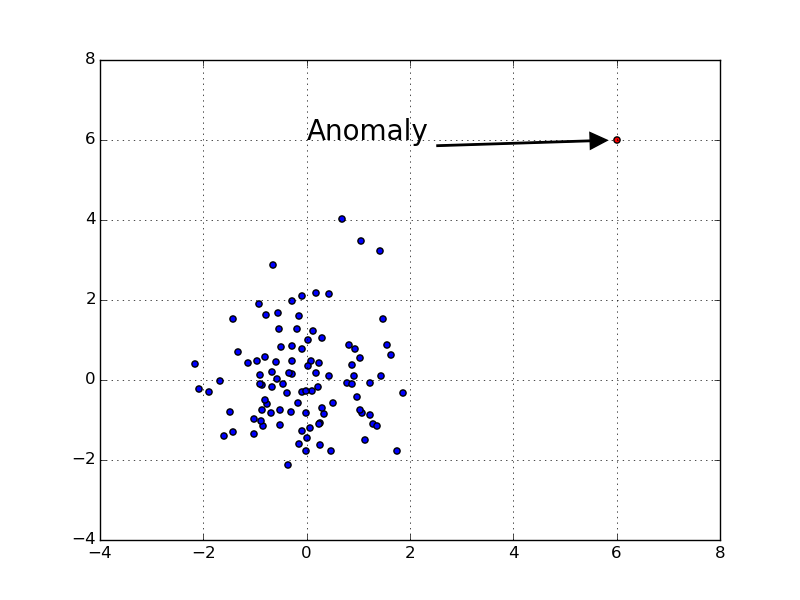
\includegraphics[scale=0.45]{anomaly_example}
\end{center}
\end{frame}

\subsection{Формальное определение}
\begin{frame}\frametitle{Формальное определение}
\begin{columns}[T]
\begin{column}{6cm}
\begin{itemize}

\item Пусть $Q$ некоторый механизм порождения данных
\item $X_1\ldots X_n$ порождены механизмом $Q$
\item $\tilde{X}_1 \ldots \tilde{X}_m$ порождены каким-либо иным механизмом
\item Тогда будем считать, точки $X_1\ldots X_n$ \textbf{нормальными} измерениями, а точки $\tilde{X}_1 \ldots \tilde{X}_m$ \textbf{аномалиями}
\end{itemize}
\end{column}
\begin{column}{6cm}
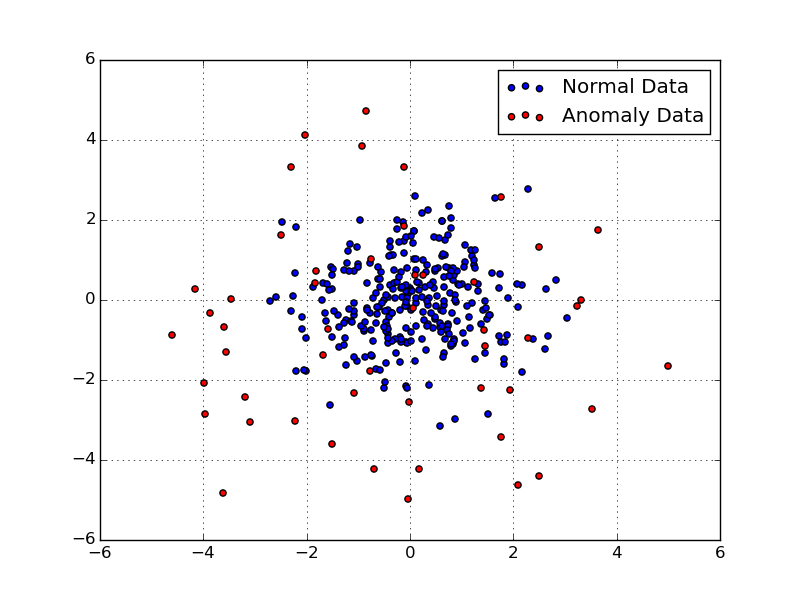
\includegraphics[scale=0.3]{uniform_anomaly_example.png}
\end{column}
\end{columns}
\end{frame}
\section{Методы детектирования аномалий}
\subsection{Краткий обзор}

\begin{frame}


\end{frame}
\end{frame}
\end{document}